\documentclass[a4paper, 12pt]{article}
\usepackage[a4paper,hmargin={3cm,2.5cm},vmargin={2.5cm,2.5cm}]{geometry}
\usepackage{amsfonts} % if you want blackboard bold symbols e.g. for real numbers
\usepackage{graphicx} % if you want to include jpeg or pdf pictures
\usepackage{multicol}
\usepackage{lipsum}
\usepackage{subfig}
\usepackage{float}
\usepackage{blindtext}
\usepackage{fancyhdr}
\usepackage{tikz}
\usetikzlibrary{calc}
\usepackage{eso-pic}
\usepackage{lipsum}
\usepackage{listings}
\usepackage{xcolor}
\usepackage{gensymb}
\usepackage{indentfirst}
\usepackage{longtable}
\usepackage{amsmath}
\usepackage{siunitx}

\lstdefinelanguage[mips]{Assembler} {
morekeywords={[1]movlw, incfsz, decfsz, movwf, movf, goto, call, sublw, addwf, andwf, return, decf, btfss, xorwf, clrf, subwf, nop, retlw, btfsc},
morekeywords={[2]org, macro, dt, endm, equ},
morekeywords={[3] STATUS, PCL},
morecomment=[l]\;,
}

\definecolor{CommentGreen}{rgb}{0,.6,0}
\lstset{
	language=[mips]Assembler,
	escapechar=@, % include LaTeX code between `@' characters
	keepspaces,   % needed to preserve spacing with lstinline
	basicstyle=\footnotesize\ttfamily\bfseries,
	commentstyle=\color{CommentGreen},
	stringstyle=\color{cyan},
	showstringspaces=false,
	keywordstyle=[1]\color{blue},    % instructions
	keywordstyle=[2]\color{red}, % directives
	keywordstyle=[3]\color{magenta},     % registers
}
\begin{document}
%========================================================= %
%================begin of title page====================== %
% The frontmatter environment for everything that comes with roman numbering\
%============================================= %
\newenvironment{frontmatter}{}{}
\begin{frontmatter}
%%%%%%%%%%%%%%%%%%%%%%%%%%%%%%%%%%%%%%%%%%%%%%%%%%%%%%%%%%%%%%%%%%%
\begin{titlepage}
%\AddToShipoutPictureBG
\begin{center}
\textup{\textbf{\large THE UNIVERSITY OF JORDAN}\textbf{}}\\[0.5cm]\textbf{\large DEPARTMENT OF COMPUTER ENGINEERING}\\[1.5cm]

%---------------------------------Figure------------------------------

\begin{center}
\begin{figure}[h]  %h means here other options t , b, p, etc.
\centering

\includegraphics[width=0.3\linewidth]{./logo1}
\end{figure}
\end{center}

%----------------------------
\begin{LARGE}
{\textbf {Embedded Systems Lab Report\\[0.5cm] Oxygen Therapy Controller}}\end{LARGE}\\[1cm]
\textit{SUBMITTED BY}\\[0.3cm]
\begin{large}
\textbf{Ehab Younes (0174788)}\\[0.1cm]
\textbf{Zeyad Al Najjar (0175642)}\\[1cm]
\end{large}
\textit{TO INSTRUCTORS}\\[0.3cm]
\begin{large}\textbf{PROF. Iyad Jafar}\\[0.3cm]\end{large}
\begin{large}\textbf{ENG. Rawan Al-Jamal}\\[0.3cm]\end{large}
\textbf{(Spring 2020-2021)}
\vfill
\end{center}
\end{titlepage}
%----------------------ACKNOWLEDGEMENT---------------------------
\pagenumbering{gobble}

\pagenumbering{roman}
\setcounter{page}{1}
\newpage
\tableofcontents
%================================================ %
% The frontmatter environment for everything that comes with roman numbering %
\end{frontmatter}
%%%%%%%%%%%%%%%%%%%%%%%%%%%%%%%%%%%%%%%

\newpage
\pagenumbering{arabic}
%%%%%%%%% MAIN TEXT STARTS HERE %%%%%%%%%%
\section{Introduction}
As per specification, the system presented here is used in hospitals to track and regulate the amount of oxygen used for oxygen therapy. This specific system was designed to accommodate only two beds. \\

\par There are three main functionalities that the system performs. First, it interactively controls the oxygen flow for each bed, depending on the need, using control knobs (potentiometers) with the option to turn off the machine for either or both beds. The second functionality is interfacing the oxygen pump and producing the correct voltages for the pump to be able to deliver the total required oxygen flow. The final and third functionality is the tracking of the amount of oxygen in the tank and notifying the user when the amount falls beyond a specified volume. \\

\par The user can interact with the system either by using the potentiometers as described above to change the flow rate or by flipping the switches to toggle the oxygen for a certain bed. Alternatively, the user can also see the amount of oxygen left in the tank by switching the LCD View switch they can see whether the system is on or off and the individual flow rate for each bed. \\

\par The oxygen tracker can also turn on an alarm (modeled by a red LED) to notify the user that the oxygen volume is low and that the tank must be refilled.

\section{System Description}
\subsection{Subsystems}
\par The system can be split into four different subsystems, each performing a specific functionality:
\begin{itemize}
  \item \textbf{Rate Control Knobs}: Two different potentiometers are used to control the flow rate of the oxygen for each bed. The potentiometer for bed1 is connected to RA0/AN0, while the potentiometer for bed2 is connected to RA1/AN1. For the values of $V_{s1}$ and $V_{BAT}$, we have chosen $V_{s1} = 5V$ and $V_{BAT} = 0V$. We also connected them to RA3/Vref+ and RA2/Vref-, respectively, for more accurate conversion.

  \item \textbf{LCD}: This subsystem displays the volume of oxygen left in the tank. It can also display the flow rate and whether the system is turned on for each bed. The LCD (model LM016L) uses the Hitachi HD44780 controller. So, RC5 - RC7 were connected to RS, RW, and E respectively which can be used to configure the LCD mode of operation. While RD0 - RD7 were connected to the data pins of the LCD to send ASCII characters and the actual configuration commands.

  \item \textbf{Pump}: The pump is responsible for delivering the oxygen rate required from both beds. The pump is represented as a 20V DC motor that can only run at a constant speed. To control the speed of the pump, the pulse-width modulation technique is used where the pump is switched on and off periodically at a high frequency to achieve an average voltage that will run the pump at the required speed.

  \item \textbf{Oxygen Volume Tracker}: This subsystem keeps track of the oxygen volume available in the tank. That’s achieved by tracking the consumption rate of both beds and updating the oxygen volume periodically. This information is displayed on the LCD in Mode 1. It’s also used to decide when to trigger the alarm mode that turns on the alarm LED and displays a warning message on the LCD.
\end{itemize}


\par
When integrating the system, we used the Timer 1 module to calculate a 1-second delay. By setting the prescale to the maximum possible (8) and
\begin{equation*}
	TMR1 = \num[group-separator={,}]{62500}
\end{equation*}


We only need 2 iterations of the timer. 

\begin{align*}
	Prescale \times TMR1 \times Counter &= Total \: Count  \\
	8 \times \num[group-separator={,}]{62500} \times 2 &= \num[group-separator={,}]{1000000}
\end{align*}

\newpage

\section{Hardware System}
\subsection{Rate Control Knobs}
When configuring the ADC we also connected the Vref+ and Vref- for more accurate values. 
This has the added advantage of making the values of $V_{s1}$ and $V_{BAT}$ arbitrary (within reason), since as long as we connect $V_{s1}$ to Vref+ and $V_{BAT}$ to Vref-, we’ll always read the same value from the ADC. 

\begin{figure}[H]
\centering
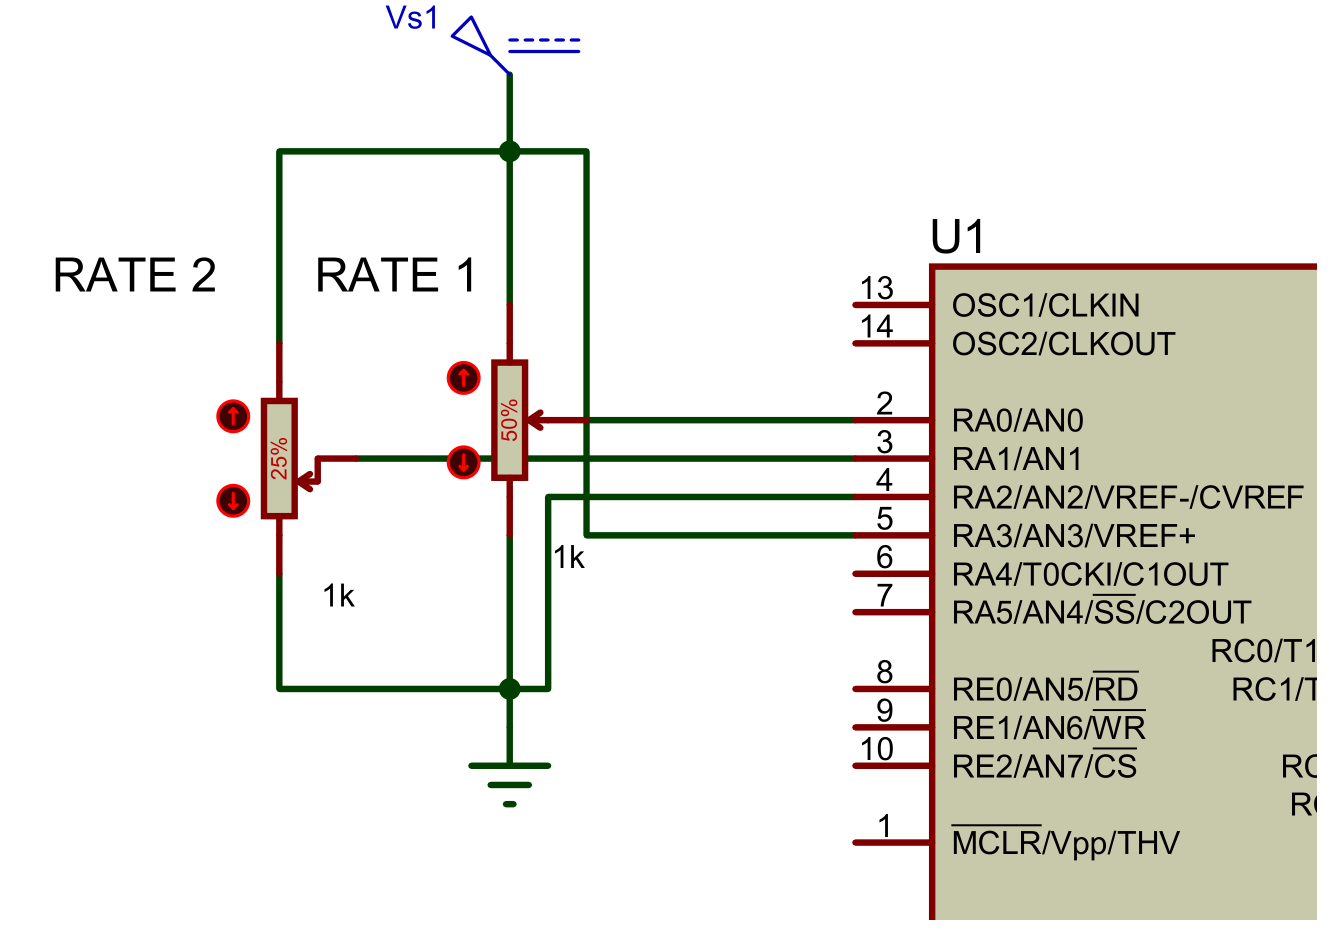
\includegraphics[width=0.8\linewidth]{images/ADC} %Change This Image
\caption{Control Knobs Circuit}
\end{figure}

\par Given these values, the resolution:

\begin{equation*}
	Resolution = \frac{5}{2^8} = 19.53125 mV
\end{equation*}

We can then find the ADC result that corresponds to the voltage by the following:

\begin{equation*}
	ADC \: Result = \frac{V_{in}}{Resolution}
\end{equation*}

\begin{figure}[H]
\centering
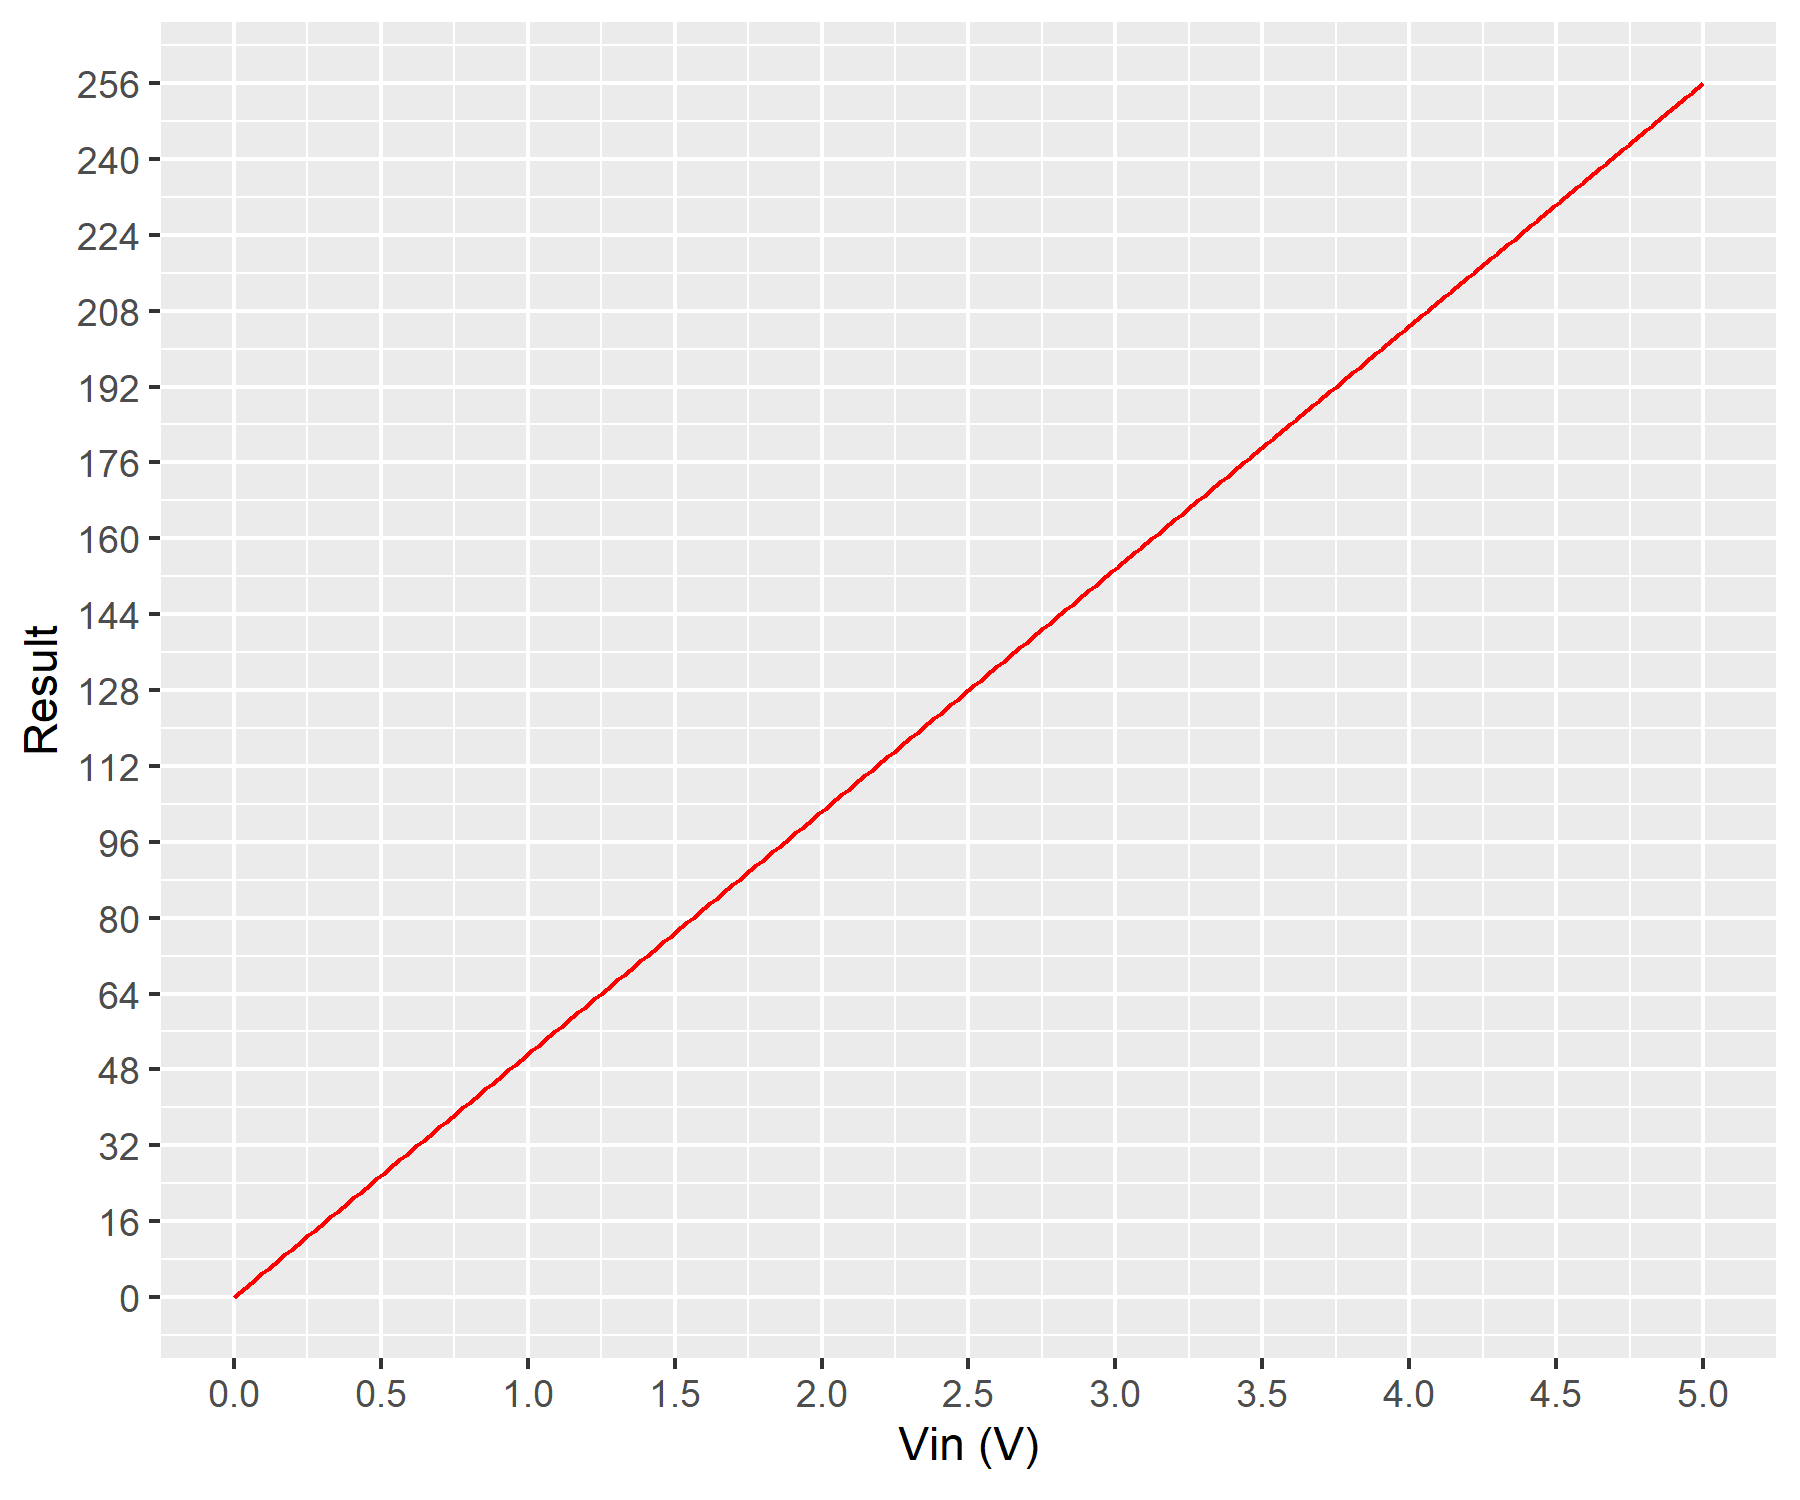
\includegraphics[width=0.9\linewidth]{images/plot}
\caption{ADC Result vs. $V_{in}$}
\end{figure}

\begin{table}[h]
\begin{center}
 \def\arraystretch{1.5}
 \begin{tabular}{|c|c|c|} 

 \hline
 Voltage (V) & ADC Result (8-bit) & Oxygen Rate (Liter/sec) \\ [0.5ex] 
 \hline\hline
 $V_{pot} = 0 $ & ADRESH = 0 & 0 \\ 
 \hline
 $0 < V_{pot} \leq 1.25$ & $0 < ADRESH \leq 64$ & 1 \\ 
 \hline
 $1.25 < V_{pot} \leq 2.5$ & $64 < ADRESH \leq 128$ & 5 \\ 
 \hline
 $2.5 < V_{pot} \leq 5$ & $128 < ADRESH \leq 255$ & 10 \\ [1ex] 
 \hline
\end{tabular}\caption{ADC Result to Oxygen Flow Rate}
\end{center}
\end{table}

Now that we have the digital value (ADRESH). We can compare the key values by subtracting then returning the required oxygen rate in the working register.

\begin{lstlisting}
GET_RATE
    movwf	ADC_VALUE
    sublw 	.128
    btfss	STATUS,    C
    retlw	.10            		; ADC_VALUE > 128
    movf	ADC_VALUE, W
    sublw	.64            
    btfss	STATUS,    C
    retlw	5           		; 128 >= ADC_VALUE > 64
    movf	ADC_VALUE, W
    btfss	STATUS,    Z
    retlw	1            		; 64 >= ADC_VALUE > 0
    retlw	0            		; ADC_VALUE = 0
\end{lstlisting}



\subsection{LCD}

\par The main basic functions of the LCD were the SEND\_CHAR which sends an ASCII character to be printed at the current cursor location, and SEND\_CMD which changes the configuration of the LCD (To clear the display or change the cursor location). \\

\par However, the interesting part of the subsystem is perhaps the subroutine DISPLAY\_STR, which prints a C-style string, meaning it keeps printing to the display until it encounters NIL or 0x00. \\

This, along with the STR\_LOOKUP that returns a character based on the display mode (Mode 1, Mode 2, and Alarm Mode). It is done by performing PCL + CURRENT\_MODE which moves the PC to the actual lookup table. \\

\begin{lstlisting}
STR_LOOKUP
    movf	CURRENT_MODE, W
    addwf	PCL, F
    goto	MODE_1_LOOKUP
    goto	MODE_2_ON_LOOKUP
    ...

MODE_2_ON_LOOKUP
    movf	STR_INDEX, W
    addwf	PCL, F
    dt		"Bed", 0x00
    dt		" ON  ", 0x00
    dt		" L/s", 0x00
\end{lstlisting}

Now the higher level subroutine simply prints the strings and fills the required custom data in between the strings, like, the bed number, the flow rate, or the oxygen volume. \\

Another interesting subroutine is the GET\_BCD\_BIG (and GET\_BCD\_SMALL) which converts a number to packed BCD. Using the inexpensive “Double Dabble” algorithm that only requires shifting and adding 3. \\

Since the oxygen volume requires more than 8-bits it was split into OXYGEN\_VOLUME\_LO and OXYGEN\_VOLUME\_HI, then arithmetic and logical operations are done first on the low-byte then the high-byte while taking care to propagate the carry (See GET\_BCD\_BIG and SUB16).

\newpage

\subsection{Pump}
As mentioned earlier, the PWM technique works by alternating the signal between high and low at a high frequency. The total time for each cycle is called the period (T) and the percentage of time the signal stays high (ton) is called the duty cycle. This can be shown in the following graph:

\begin{figure}[H]
\centering
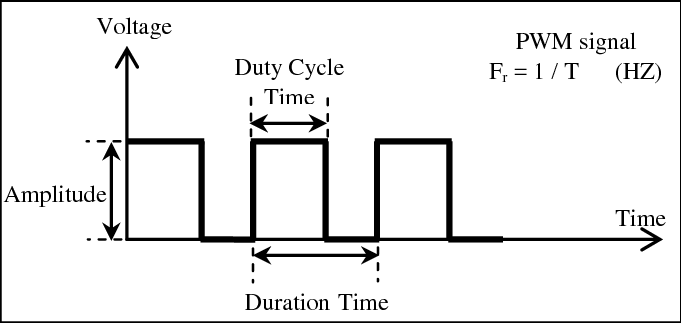
\includegraphics[width=0.8\linewidth]{images/PWM}
\caption{PWM}
\end{figure}

By adjusting the duty cycle, we can change the average voltage applied to the motor to achieve the required speed for the pump.  \\

Another important point to mention is that the pump operates at 20 volts whereas the PIC microcontroller can only provide 5 volts so, we used an N-Channel MOSFET (2N6660) to be able to control the pump through the following circuit:

\begin{figure}[H]
\centering
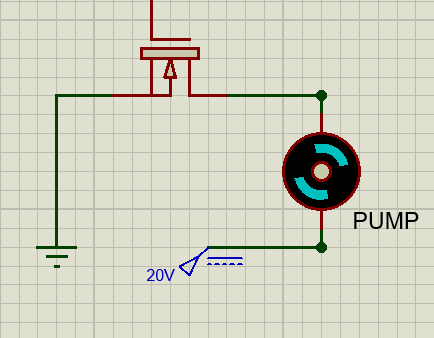
\includegraphics[width=0.5\linewidth]{images/MOSFET}
\caption{Pump Circuit}
\end{figure}

When the microcontroller outputs a high signal, the transistor switches on connecting the motor to the ground and completing the circuit which lets the current pass through the pump switching it on. When the output is set to low, the transistor goes into the cutoff mode which creates an open circuit and disconnects the circuit switching the pump off. \\

Now, each oxygen rate range is achieved by setting the pump to work at a specific speed. These values are shown in Table~\ref{tab:rate_rpm}.
\begin{table}[h]
\begin{center}
 \def\arraystretch{1.5}
 \begin{tabular}{|c|c|c|} 

 \hline
 Total Oxygen Rate (Liter/sec) & Speed (RPM) \\ [0.5ex] 
 \hline\hline
 $Rate = 0$ & 0 \\ 
 \hline
 $0 < Rate \leq 5$ & 10 \\ 
 \hline
  $5 < Rate \leq 10$ & 40 \\ 
 \hline
  $10 < Rate \leq 15$ & 70 \\ 
 \hline
  $15 < Rate \leq 20$ & 100 \\ [1ex] 
 \hline
\end{tabular}\caption{Rate to RPM} \label{tab:rate_rpm}
\end{center}
\end{table}

The required voltage to be applied to the pump to achieve these speeds can be calculated with:

\begin{equation*}
    V_{avg} = \sqrt{\frac{speed}{4}}
\end{equation*}

To get these voltages, we need to use appropriate values for the period and duty cycle. We chose a period of 1/2500 seconds giving us a frequency of 2.5KHz which after testing appeared to be the best option for both stability and accuracy. The period is fixed for all speed levels whereas the duty cycle varies. The duty cycle is calculated with: 

\begin{equation*}
    Duty \: cycle = \frac{V_{avg}}{20} \times 100\%
\end{equation*}

Now, we can use these percentages to calculate the ton which is the amount of time the signal stays on:

\begin{equation*}
    t_{on} = Duty \: cycle \times T
\end{equation*}

These calculations are shown in Table~\ref{tab:pwm_calculations}.
\begin{table}[h]
\begin{center}
 \def\arraystretch{1.5}
 \begin{tabular}{|c|c|c|c|} 

 \hline
 Speed (RPM) & $V_{avg}$ (V) & Duty cycle $(\%)$ & $t_{on} (\mu S)$ \\ [0.5ex] 
 \hline\hline
 0 & 0 & 0 & 0 \\ 
 \hline
10 & 1.58 & 7.9 & 32 \\ 
 \hline
  40 & 3.16 & 15.8 & 63 \\ 
 \hline
 70 & 4.2 & 20.9 & 83 \\
\hline
100 & 5 & 25 & 100\\ [1ex] 
 \hline
\end{tabular}\caption{PWM Calculations} \label{tab:pwm_calculations}
\end{center}
\end{table}


\subsection{Oxygen Volume Tracking}
This subsystem is responsible for tracking the consumption of oxygen and the available oxygen volume. It works by updating the oxygen volume each cycle, subtracting the total oxygen rate for that cycle from the oxygen volume. \\

It then checks if the remaining volume is less than the alarm volume (500) and if so, it sets the alarm flag to high which alerts the LCD subsystem to display the warning message. \\

Both of these operations introduced a bit of a challenge because the oxygen volume is a 16-bit value and the PIC microcontroller doesn’t support 16-bit operations (see the obstacles section). \\

Both the Max Oxygen Volume, which the oxygen volume is initialized to and is set to when the fill button is clicked, and the Alarm Volume are stored in constants that can be easily changed in case the system has to be deployed in different environments. \\


\newpage

\section{System Testing and Results}
At first, each individual subsystem was implemented and tested on its own. \\

\subsection{Rate Control Knobs}

Since the first thing we implemented was the LCD, we were able to actually print the register values to the LCD to test it. \\

Here are some various percentages of both knobs (0\%, 25\%, 50\%, and 100\%). As we can see the values are correct. \\

\begin{figure}[H]
\centering
\begin{minipage}{.5\textwidth}
  \centering
  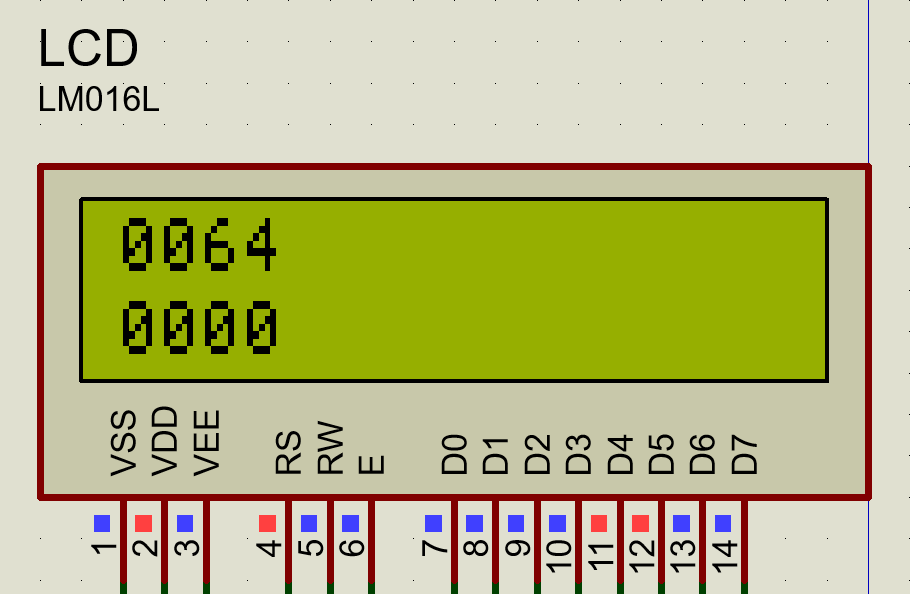
\includegraphics[width=0.95\linewidth]{images/ADC_Test1}
  \captionof*{figure}{Rate1 at 25\% and 0\%}
\end{minipage}%
\begin{minipage}{.5\textwidth}
  \centering
  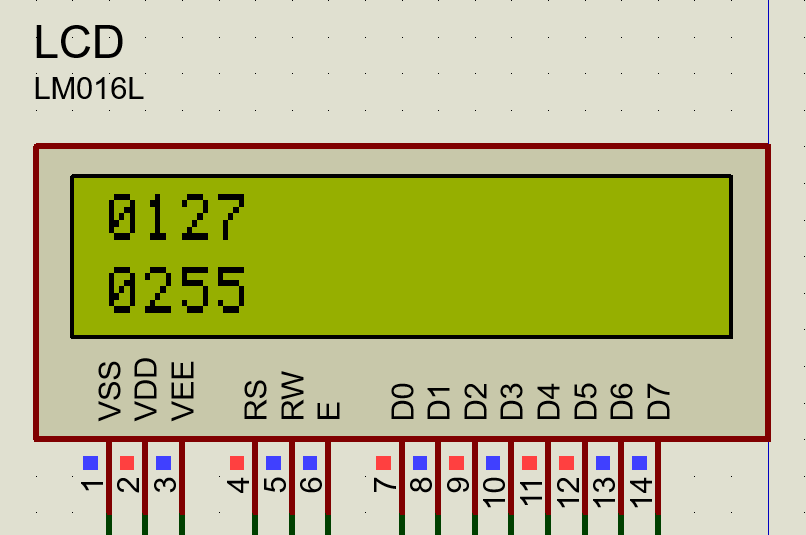
\includegraphics[width=0.95\linewidth]{images/ADC_Test2}
  \captionof*{figure}{Rate1 at 50\% and 100\%}
\end{minipage}
\end{figure}


\begin{lstlisting}
call	READ_ADC_VALUES
    
    	movf		ADC_VALUE1, W
    	movwf	 	NUMBER_LO
    	clrf		NUMBER_HI
    	call		GET_BCD_BIG
    	SEND_BCD	BCD_HI
    	SEND_BCD	BCD_LO
    
    	call		GO_TO_LINE2
    
	movf		ADC_VALUE2, W
    	...

\end{lstlisting}


\newpage


\subsection{LCD}
To test the DISPLAY\_STR subroutine in the LCD, we put different texts and separated them with NIL (0x00) then tried to call DISPLAY\_STR various times to see if it prints the required string. \\

For example, if we execute this code then we expect it to NOT print the “4th” string, since it is not reached:

\begin{lstlisting}
	clrf    	   STR_INDEX
    	call    	   DISPLAY_STR_TEST    	; 1st string
    
    	call    	   GO_TO_LINE2
     
    	call    	   DISPLAY_STR_TEST    	; 2nd string
   	call    	   DISPLAY_STR_TEST	; 3rd string
    	movlw    	   0xD2
	movwf    	   NUMBER_LO
	movlw    	   0x04  
	movwf    	   NUMBER_HI        	; 0x04D2 = (1234) base 10
	call    	   GET_BCD_BIG
	SEND_BCD    BCD_HI
	SEND_BCD    BCD_LO

TEST_LOOKUP
    	movf    	   STR_INDEX, W
    	addwf    	   PCL, F
    	dt        	   "Text on line1", 0x00
    	dt        	   "2nd", 0x00
    	dt         	   "3rd", 0x00
    	dt        	   "4th", 0x00

\end{lstlisting}

\begin{figure}[H]
\centering
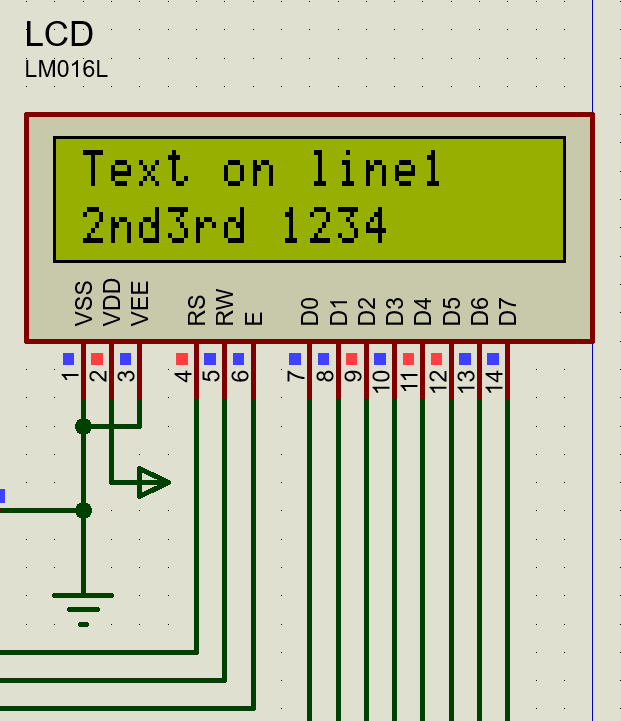
\includegraphics[width=0.45\linewidth]{images/LCD_Test}
\caption{LCD Test}
\end{figure}

Notice also that 0x04D2 which is 1234 in base 10 has also been printed correctly.


\subsection{Pump}

To make sure our calculations are correct and the pump subsystem is working as expected, we used an AC voltmeter which measures the RMS voltage of the pump. \\

\begin{figure}[H]
\centering
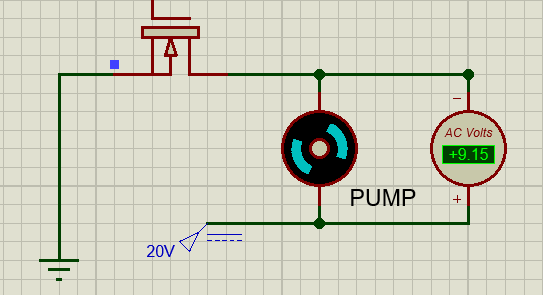
\includegraphics[width=0.45\linewidth]{images/Pump_Test}
\caption{Pump Test}
\end{figure}

Then we used this value to calculate the duty cycle with the following formula:
\begin{equation*}
	V_{RMS} = \sqrt{\frac{1}{T} \int_{0}^T f(t)^2 dt}
\end{equation*}

Since this is a square wave that is either 20V or 0 (Assuming $ON$ is from 0 to $t_{on}$):
\begin{equation*}
	V_{RMS} = \sqrt{\frac{1}{T} \int_{0}^{t_{on}} 20^2 \: dt}
\end{equation*}


Finally:
\begin{equation*}
	Duty \: cycle  = \frac{t_{on}}{T} \times 100\% = \frac{V_{RMS} ^ 2}{400} \times 100\%
\end{equation*}
After that, we compared the measured values of the duty cycle with the theoretical values and made sure they’re all within the margin of error. \\

\newpage


\subsection{System Integration}
Finally, after testing each subsystem fully, we created the system by combining all the subsystems. Which was then tested as per the project specification.

\begin{figure}[H]
\centering
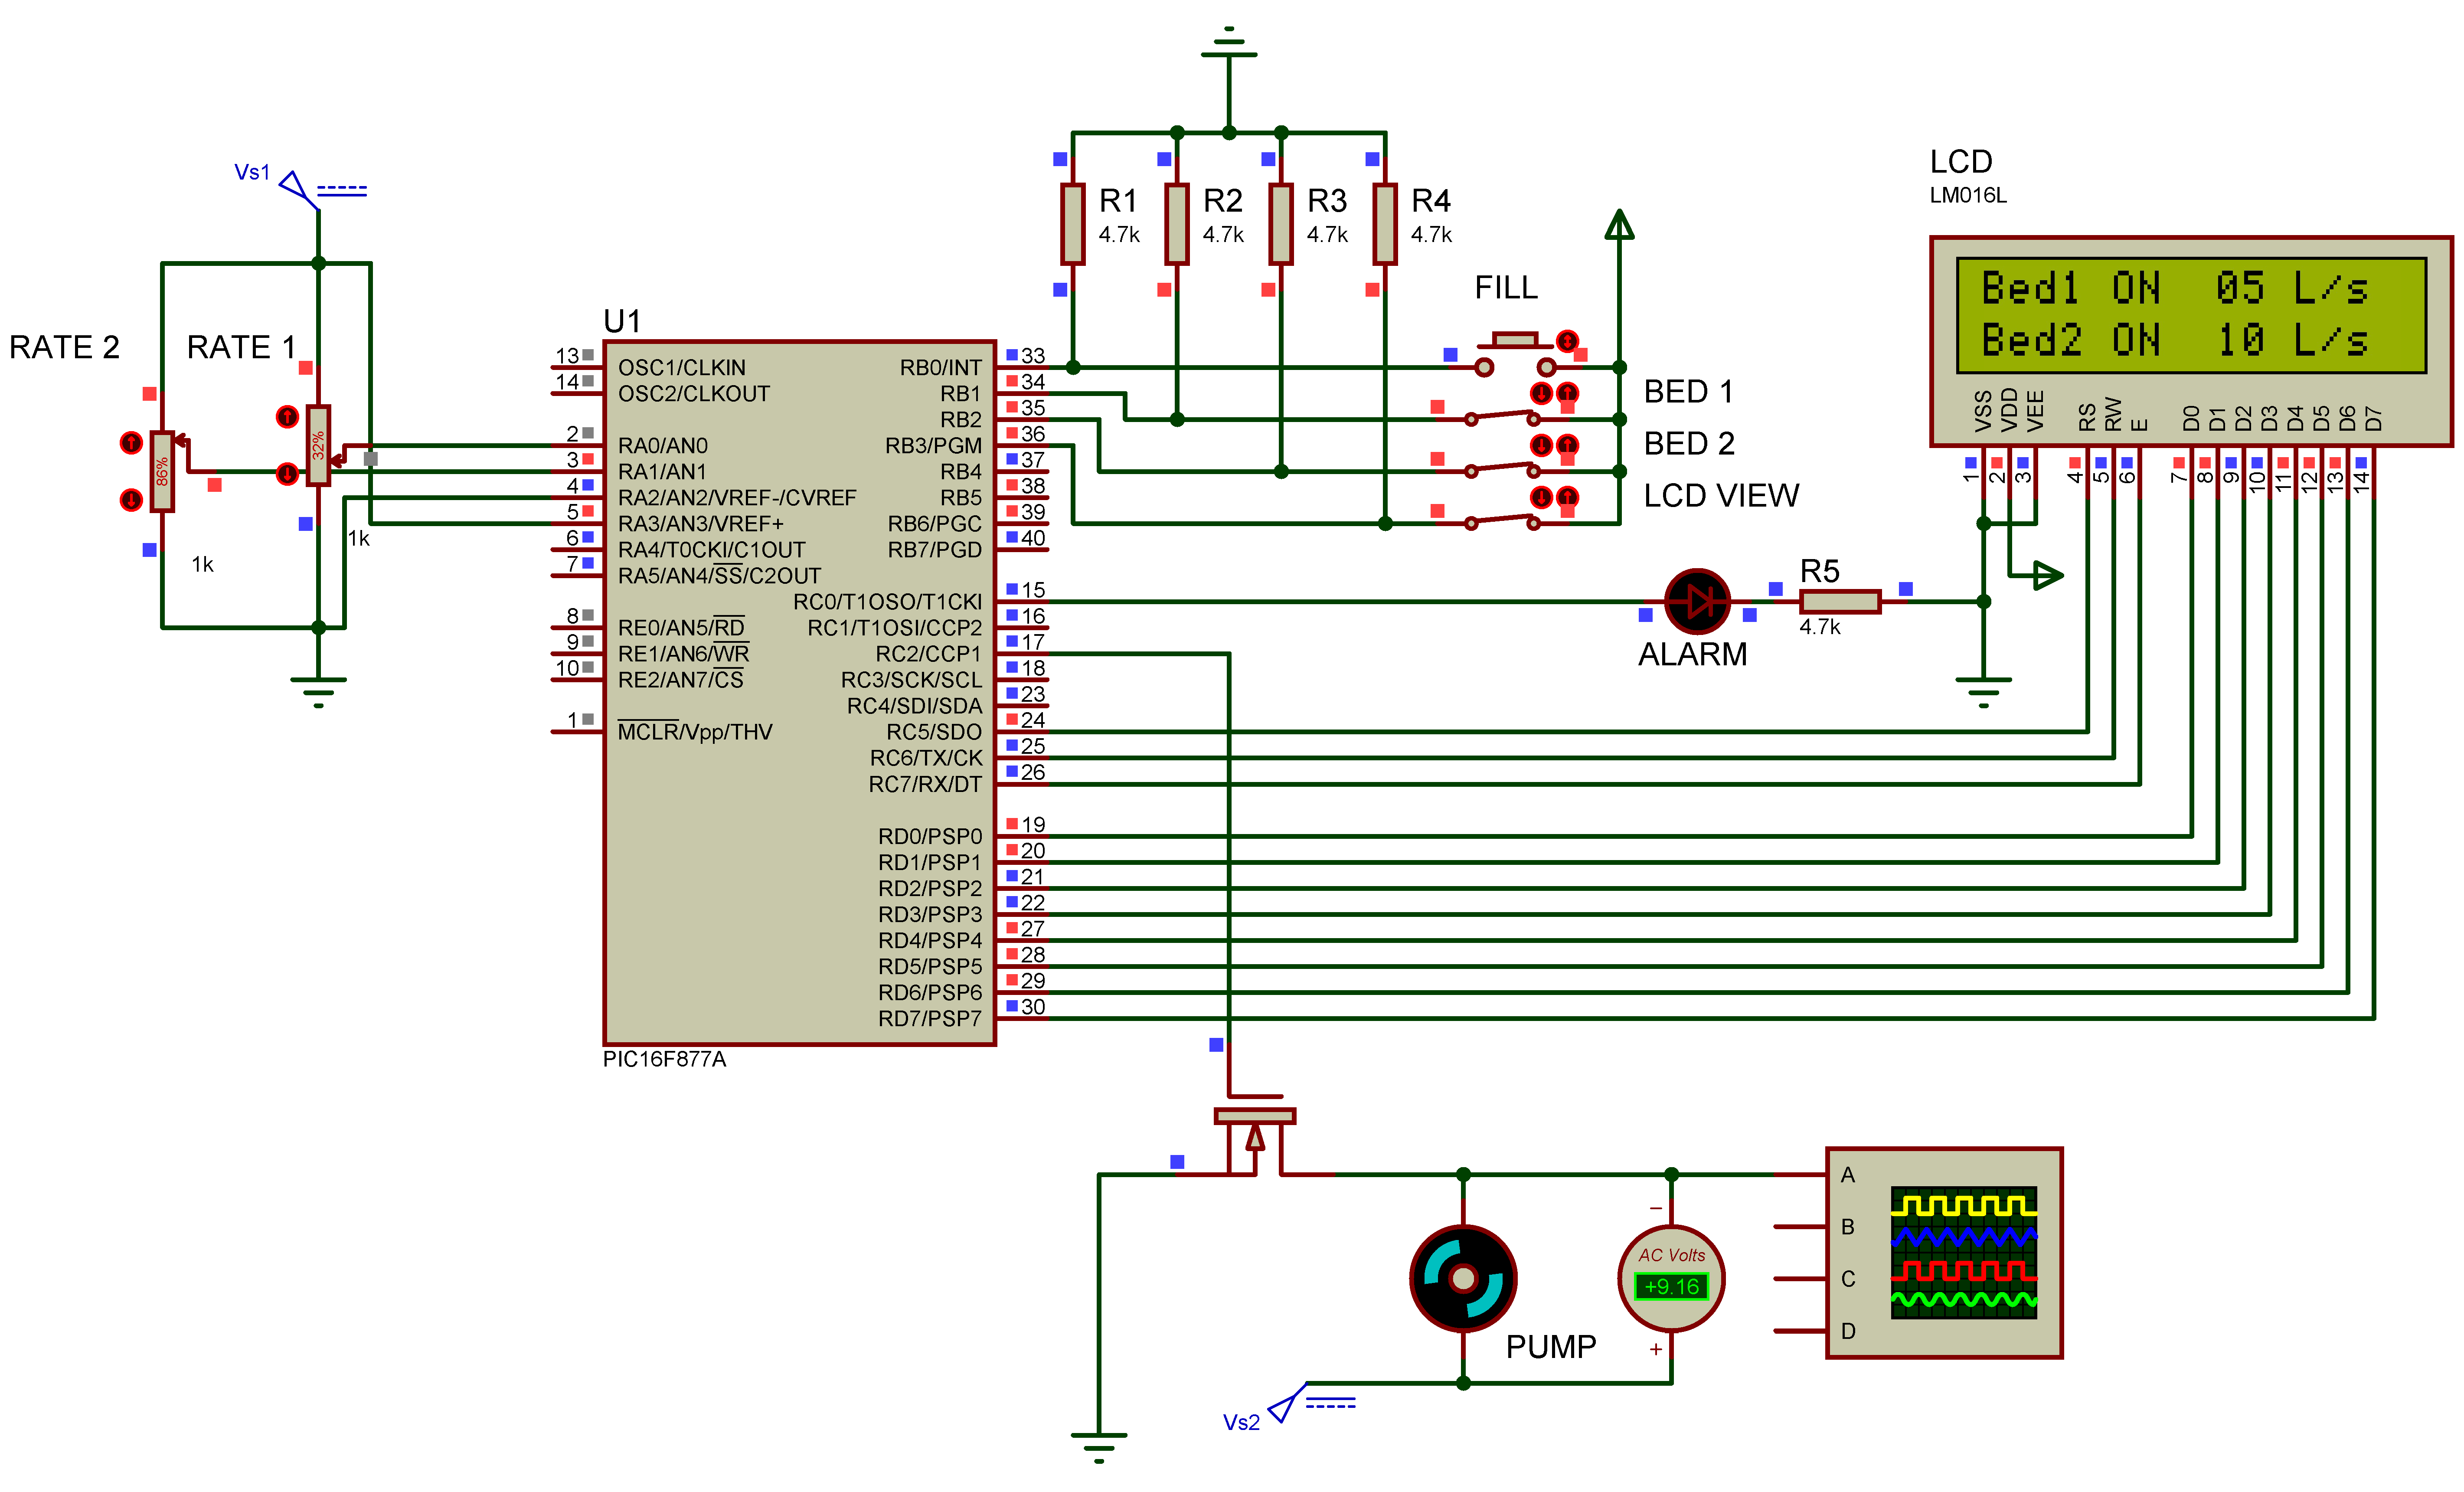
\includegraphics[width=\linewidth]{images/FullSystem}
\caption{Full System Design}
\end{figure}

Here, we tested different input combinations, toggled all the switches and pushed the button. Everything was working correctly as specified.

\newpage

\section{Conclusion}

\subsection{Summary}
\par At the end of this project, we had a fully functional oxygen therapy system with the option to track the oxygen volume, the oxygen flow rate, control the pump, and notify the user when the tank is running low. The software was modularly designed such that each module or subsystem is independent of the other. This made testing, integration, and modification much easier and more straightforward. \\

Regarding the hardware, the system design is simple and efficient. All of the components are cheap and readily available, while also the power consumption is low. \\

Notice how the PROCESS subroutine actually calls each individual subsystem, then in each subsystem there functionality is also split into multiple subroutines. \\

\subsection{Contributions}
\par Since we had 4 different subsystems, we each took 2 subsystems to work on:
\begin{itemize}
  \item \textbf{Rate Control Knobs and LCD}: Ehab Younes
  \item \textbf{Pump and Oxygen Volume Tracker}: Zeyad Al Najjar
\end{itemize}

\par System integration and testing was done by both of us together.

\subsection{Obstacles}
We encountered many obstacles when working on this project, here are the most prominent ones:

\subsubsection{Strings and Display Modes}
We wanted to create a single lookup table to display the required information, however, there were essentially 4 different display modes. So, instead of creating multiple subroutines and copying DISPLAY\_STR 4 different times, we used the look up trick to choose which display mode to print. Now we only have to set CURRENT\_MODE to pick the display mode, along with using STR\_INDEX to keep track of what we are printing in that display mode.


\begin{lstlisting}
STR_LOOKUP
    movf	CURRENT_MODE, W
    addwf	PCL, F
    goto    	MODE_1_LOOKUP
    goto   	MODE_2_ON_LOOKUP
    goto    	MODE_2_OFF_LOOKUP
    goto    	MODE_ALARM_LOOKUP
\end{lstlisting}


\subsubsection{16-bit Subtraction and Comparison}
There are two instances where we need to subtract from a 16-bit number. First, when subtracting the total oxygen rate from the oxygen volume. Second, when comparing to see if the oxygen volume has fallen below 500. \\

To do this operation we created a 16-bit subtraction that also produces the correct carry as described by \cite{sub16}:

\begin{lstlisting}
SUB16      	macro   DST, SRC
    movf    	(SRC), W
    subwf    	(DST), F    	; Subtract DST(low) - SRC(low)
    movf    	(SRC)+1, W       ; Now get high byte of subtrahend
    btfss    	STATUS, C        ; If there was a borrow increment SRC(high)
    incfsz    	(SRC)+1, W       
    subwf    	(DST)+1, F       ; Subtract DST(high) - SRC(high)
    endm
\end{lstlisting}

\subsubsection{Converting a Binary Number to Binary Coded Decimal (BCD)}
This was also used in two instances. First, when displaying the 16-bit oxygen volume calculated above. Second, when displaying the 8-bit oxygen flow rate. \\

To find the value of the units, tens, hundreds, and even thousands using loops can be extremely inefficient in code and performance. So I deployed the popular algorithm “Double Dabble” \cite{doubledabble} which is mainly used for simple controllers that lack a division unit. \\

Essentially, this algorithm adds 3 to a BCD digit if it’s bigger than or equal 5 before shifting left. Because in decimal $2 \times 5$ produces a 2-digit number. This operation (addition of 3 then shifting left) is done until all bits have been processed. To reduce computing even more, I left justified the bits then performed the algorithm in less iterations. \\


Here’s an example of how it works, assuming we want to convert the number $(27)_{10}$ using only the first 5 bits to BCD:

\begin{lstlisting}
0000 0000       	00011011      Initialization
0000 0000       	11011000      Left justify the lower 5 bits
0000 0001       	10110000      Shift
0000 0011       	01100000      Shift
0000 0110       	11000000      Shift
0000 1001      		11000000      Add 3 to ones, since it was 6
0001 0011       	10000000      Shift
0010 0111       	00000000      Shift (Fifth)
   2    7
\end{lstlisting}


\subsubsection{Inaccurate Timer 0}
After we integrated the system and ran a different number of scenarios. We noticed that the oxygen tank reaches 500 Liters after ~105 seconds instead of 100 seconds when the rate is 20 L/s.  \\

This was caused by TMR0 drifting off with time, and becoming more noticeable as time went by. After investigation, we found that this is mostly caused by the software counter that has a high value of $(125)_{10}$. \\

To fix this issue, we used the more accurate 16-bit Timer 1 as described above. \\

This change resulted in very high accuracy and the oxygen tank reaches the 500 Liter mark at exactly 100 seconds in the described settings. \\


\subsubsection{Stack Overflow}
Again, this issue happened when we integrated the system and had to call subroutines within subroutines. It appeared that the stack was overflowing because of 8 nested subroutine calls. To fix this issue, we implemented macros instead of subroutines when appropriate.  \\

In general, we used macros a fair amount. This is because we needed to execute certain functionalities quickly while also passing inputs and outputs without having to move values around. (See the macros at the beginning of the source code) \\



\begin{thebibliography}{10}

\bibitem{sub16}
  Rudy Wieser,
  \textit{16-bit Subtraction with Borrow},
  PICList, 
  viewed 21 May 2021,
  \textless http://www.piclist.com/techref/microchip/math/sub/16bb.htm\textgreater

\bibitem{doubledabble}
  \textit{Double Dabble},
  Wikipedia, 
  viewed 16 May 2021,
 \textless https://en.wikipedia.org/wiki/Double\_dabble\textgreater

\end{thebibliography}


\end{document} 

